\documentclass[11pt]{amsart}
%Include Necessary Packages
%\input{HelperFiles/include_packages}
\usepackage{geometry}
\usepackage{pdfpages}               
\usepackage{graphicx}
\usepackage{amssymb}
\usepackage{epstopdf}
\usepackage{setspace}
\usepackage{natbib}
\usepackage{hyperref}
\usepackage{comment}
\usepackage{float}

\DeclareGraphicsRule{.tif}{png}{.png}{`convert #1 `dirname #1`/`basename #1 .tif`.png}
\geometry{letterpaper}               
%\geometry{landscape}             % Activate for for rotated page geometry
%\usepackage[parfill]{parskip}    % Activate to begin paragraphs with an empty line rather than an indent
%\doublespacing 					
\def\ci{\perp\!\!\!\perp}
\def\nci{\ci\!\!\!\!\!\!\//}

\title{Crime Reduction Benefits of ABC}
\date{March 24, 2014}

\begin{document}

\maketitle

%\input{1_intro}
\section{Intro}
No study has ever evaluated comprehensively the impact of ABC on crime before. The only previous Cost-Benefit study \citep{barnett2007comparative}, only used self-reported youth data. In this report, we gather all available sources of information and comprehensively calculate the impacts of the ABC program on number and costs of crimes. We find important reductions in both the numbers and the total costs from crime for the treatment group. The total cost savings due to crime reduction are around \$120,000 per individual (2014 US dollars). 

\section{Our Data}
We use all the crime data available for ABC. It comes from several different sources: (i) Administrative data on offenses, gathered for the age-21 follow-up; (ii) Administrative data on offenses, gathered for the age-30 follow-up; (iii) Administrative data on sentences, gathered for the age-30 follow-up; (iv) Self-reported data. As none of those data sources are comprehensive of all crimes committed, it is necessary to combine them to have a complete perspective on the total magnitude of crime. In our crime analysis, we also use data from the National Crime Victimization Survey (NCVS), North Carolina Department of Public Safety (NC DPS), Bureau of Justice Statistics (BJS), National Judicial Reporting Program (NJRP), and Uniform Crime Reporting (UCR). 

\section{Methodology}
We now explain the steps used in our calculations.

1. \textbf{Fill out Missing Data:} There is missing information regarding arrests at adult age for a few individuals. We know this because there are sentences for which we do not observe the corresponding arrests. While this is possible for some particular crimes such as speeding or shoplifting, it is not possible for others such as murder. Moreover, pattern show that our data on arrests is completely missing for a small number of individuals. As we have the number of sentences for all individuals in the data, we fill out missing information on arrests using the national Arrest-to-Sentences ratios for each category of crime. \\

2. \textbf{Obtain Predictions:} We use the NC DPS data for our predictions of future crime. This dataset contains all the sentences for individuals in North Carolina, and it follows individuals longitudinally. This data starts from 1972 (43 years ago), so it contains an almost complete lifetime crime histories for some cohorts of individuals. We use the earlier cohorts available in the data, and estimate a prediction model of how many crimes they committed in their later years. In particular, we estimate how many crimes will be committed at ages 35-65 based on all types of crimes committed at ages 20-35. Then, we apply these predictive models to the ABC data to obtain an estimate of the number of sentences individuals in the ABC study will receive during their lifetimes\\

3. \textbf{Victimization Inflation:} Victimization inflation is a method used to capture benefits in crime reduction for crimes that the Justice System missed. For some types of crimes, there are many more reported crimes in the US than arrests or sentences for those crimes. In this paper we assume that those ``unpunished crimes'' were committed by the same people who committed the ``punished crimes'' of the same type. For example, we might assume that all the property crimes committed in the US were perpetrated by the same people who were arrested for property crimes. We first construct national ratios of total number of punished crimes over total number of reported crimes, and then inflate each of the crimes in our data by the inverse of that ratio.\\

4. \textbf{Incorporate Costs of Crime:} There are many methods to estimate unit costs of representative crimes, and many studies estimating them. \cite{cohen2010estimating} and \cite{mccollister2010cost} give good reviews of the state of the literature. There are two general types of methodologies that are used to estimate the total costs of crime: the Top-Down methodologies and the Bottom-Up methodologies. The former attempts to quantify the value that people put in ex-ante prevention of crime, while the latter attempts to gather ex-post all sources of costs that crimes might have. We use the latter method because the literature provides cost estimates more detailed and for more types of crimes using this methodology. It is worth mentioning that the Bottom-up estimates of the costs of crime are usually lower than the top-down analogous. The costs used in this study are presented in the ``Bottom-Up'' column of Table \ref{tab:individual-crime-cost}. \\

\begin{table}[H] \caption{Unitary Costs of Crime, Excluding Sentences} \label{tab:individual-crime-cost}
\begin{tabular}{lccc}
Crime			&Top-Down Approach	&Bottom-Up Approach:&Bottom-Up Approach:\\ 
				&					&Victim				&Justice System \\ \hline \hline
Arson			&					&\$65,377			&\$2,636\\
Assault			&\$95,200			&\$12,093 			&\$3,300\\
Burglary		&\$34,000			&\$1,467 			&\$2,390\\		
Fraud			&					&\$0				&\$3,118\\
Larceny			&					&\$528 				&\$2,567\\
Vehicle Theft	&					&\$6,699 			&\$2,683\\
Murder			&\$13,192,000		&\$9,286,200 		&\$4,734\\
Rape			&\$322,320			&\$224,021 			&\$2,593\\
Robbery			&\$315,520			&\$7,273 			&\$2,861\\
Vandalism		&					&\$0				&\$2,517\\
Miscelaneous	&					&					&\$2,517\\
\end{tabular}

\footnotesize{Note: All amounts in 2014 dollars. The costs in the Top-Down column are taken from \cite{cohen2004willingness}. The costs in the Bottom-Up column are taken from \cite{cohen1994costs}, \cite{miller1996victim}, and \cite{mccollister2010cost}. Estimates from \cite{mccollister2010cost} are used only for Fraud and Vandalism.}
\end{table}

\section{Preliminary Results}

1. \textbf{Criminal Behavior:} The results show that there are clear reductions in the amount of crime committed between the control and treatment groups. This holds true for the majority of the categories of crime. The exceptions were Vehicle Theft, Assault, Robbery, and Arson. The visualization of the ABC data in Figure \ref{tab:lifehistory} represents the life history of each of the individuals within the ABC study that committed at leaast one crime, with each dot as an offense and each line as a period of incarceration. Also shown are the most serious crimes committed in the ABC data, including a habitual felon, manslaughter, and indecent liberties with children. The largest treatment effects occurred in cases of Miscellaneous, Fraud, and Larceny crimes. In sentences alone, there was a 46.3\% reduction in the number of cases, and in arrests, there was a 39\% reduction in cases for those in the treatment group compared to the control group. There are substantially fewer offenses for the individuals in the treatment group, and although there are still a few who committed a series of crimes, many did not commit any offenses at all.
%numbers from combined_datasetv3

\begin{figure} [H]
\caption{Visualization of ABC Data} 
\centering \label{tab:lifehistory}
{\scalebox{0.8}{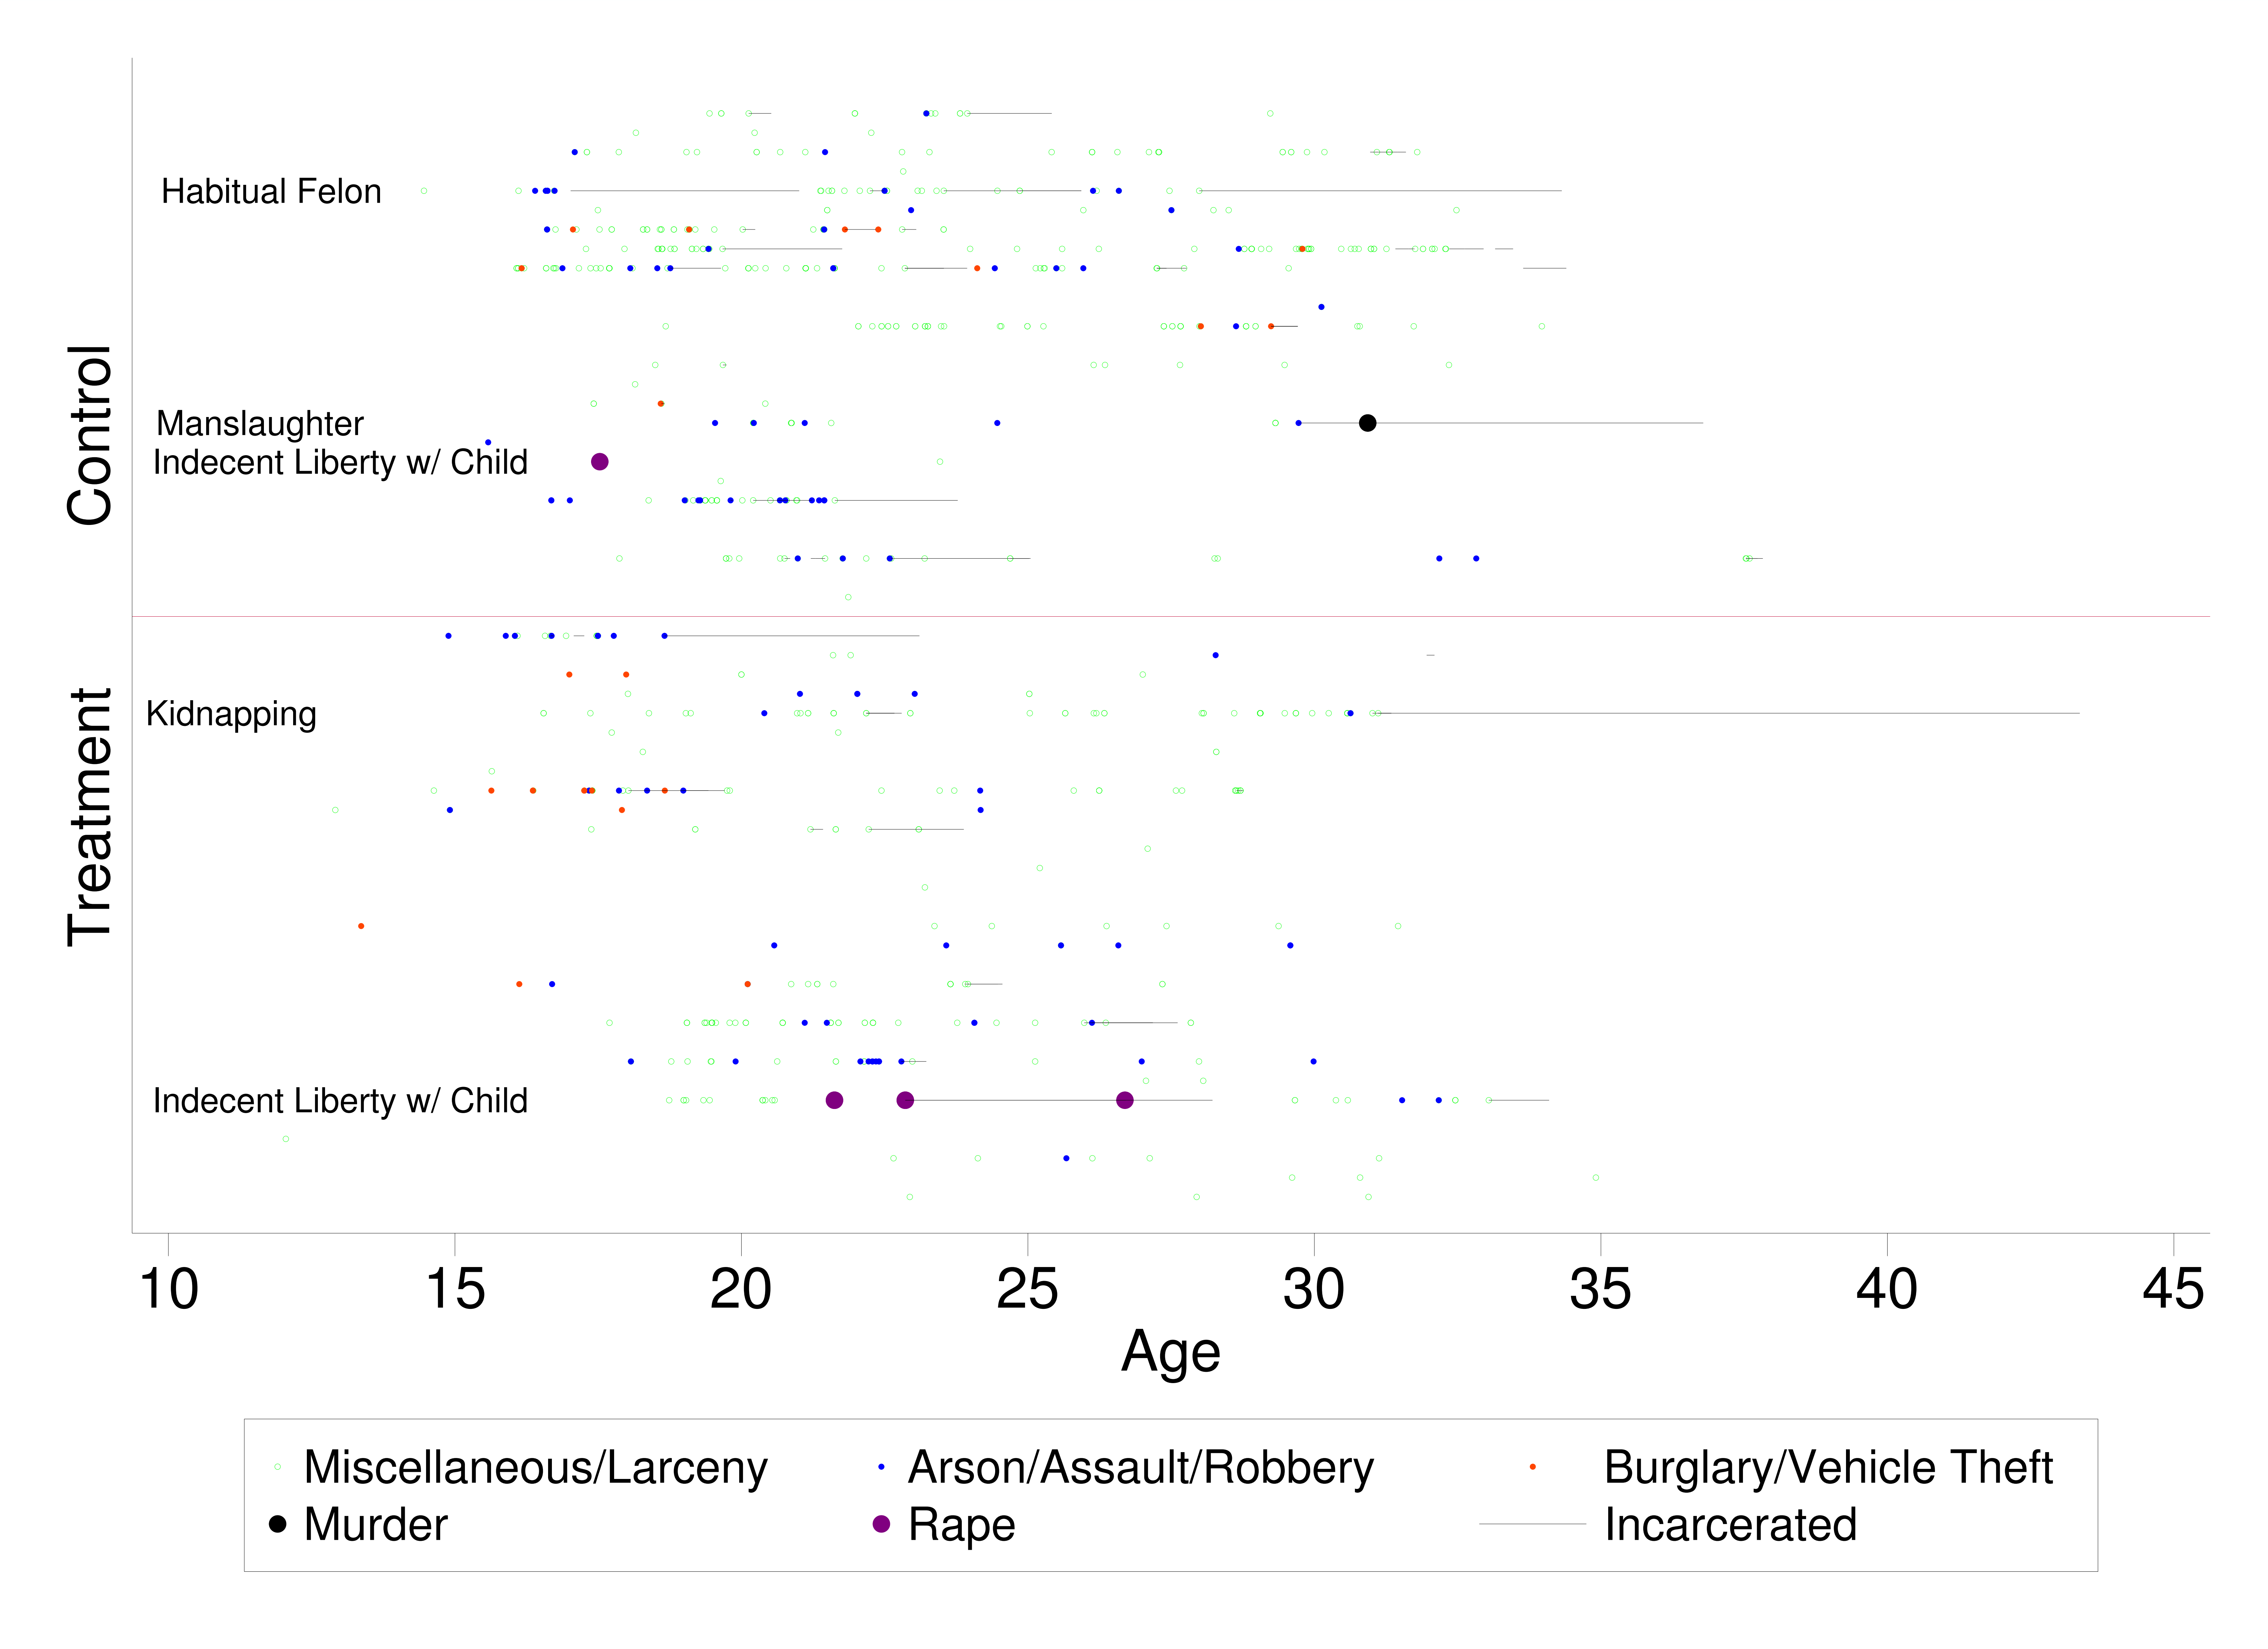
\includegraphics{lifehistory.pdf}}} 
\end{figure} 

2. \textbf{Costs of Crime:} After imputing the costs of crime and incorporating them into the data, the results are depicted in Figure \ref{tab:cost-graph}, for both before and after the Victimization Inflation. As shown below, the inflation allows us to cover a very substantial amount of crime that otherwise would have been ignored. The costs after the inflation are more than 6 times greater, with a stronger account of the categories of crimes that are typically missed by the justice system such as rape, larceny, and vehicle theft. Categories such as Murder, Rape and Vehicle Theft involved the highest costs of crime from our data, being the cause for the majority of the overall costs. Comparing the bars in Figure \ref{tab:cost-graph}, the costs from the Justice System (the treatment saves \$5740 per individual) and Imprisonment (the treatment imply additional expenditure of \$1,226 in imprisonment) are almost negligible compared to the victimization costs, even without the inflation. Yet as in Figure \ref{tab:lifehistory}, there is a clear drop in the total costs for those in the treatment group. The graph shows that the treatment saves \$118,520 to society in victimization costs.

\begin{figure} [H]
\caption{Costs of Crime After Victimization Inflation} 
\centering  \label{tab:cost-graph}
{\scalebox{0.8}{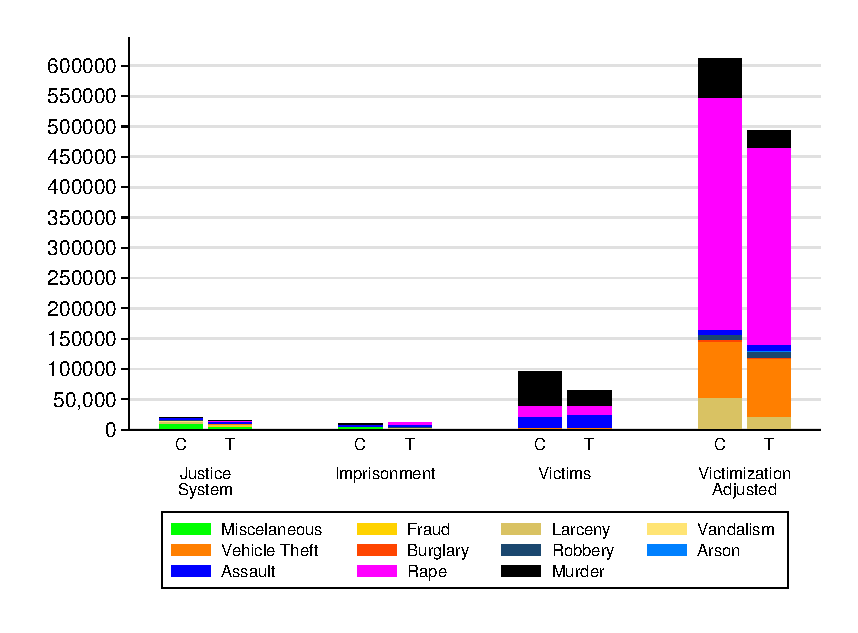
\includegraphics{Costs-vi.eps}}} 
\end{figure}

While the impacts on costs are very strong in economic magnitude (enough to pay the program on their own), they are not statistically significant. This is not surprising given the large across-individual variability of the crime costs and the  small sample of the ABC population. It is worth noting that for this study the relevant statistical significance is the one corresponding to the benefit-to-cost ratio that is calculated as final outcome of the paper. The significance of individual components is not as important.

%	Bibliography
\clearpage
\bibliographystyle{chicago}
\bibliography{AHDec5}

\end{document}
